\documentclass{homework}

\usepackage{cleveref}
\usepackage{macros}

\name{Nate Stemen}
\studentid{20906566}
\email{nate@stemen.email}
\term{Fall 2021}
\course{General Relativity for Cosmology}
\courseid{AMATH 875}

\hwname{Lecture}
\hwnum{2}
\duedate{Sun, Sep 12, 2021 9:00 PM}

\begin{document}

For me, there were three main takeaways from this lecture:
\begin{enumerate}
	\item The ideas underlying the tangent space at a point \label{it:idea}
	\item The (algebraic) definition and construction of the tangent space at a point \label{it:alg}
	\item The way in which a diffeomorphism of smooth manifolds induces a vector space isomorphism of tangent spaces \label{it:diff}
\end{enumerate}

\paragraph{\Cref{it:idea}:}
If we think of a ball travelling on a circle we use the fact that the circle's tangent vectors coincide with the ball's velocity vectors.
\begin{figure}[h]
	\centering
	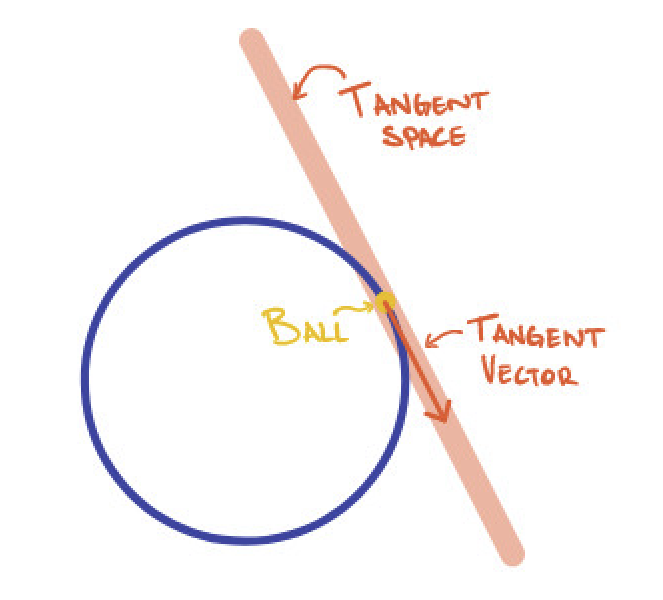
\includegraphics[width=.3\textwidth]{circle.pdf}
\end{figure}
Indeed depending on the velocity of the the tangent plane to the circle will always contain it's velocity vector and it will also be a vector space.
This idea can of course be generalized to more complicated spaces than circles and spheres and indeed that's exactly what we set out to do.

\paragraph{\Cref{it:alg}:}
This was the most fascinating part of the lecture to me as I've had a picture of the tangent space in my head, but never seen the formal construction using derivations.
What we do is look at all functions that are equal ``around'' our point of interest $p$ and make an equivalence class---in effect only leaving functions who behave differently around $p$.
We then define the tangent space $T_p(M)$ of our manifold $M$ at $p$ to be the vector space of derivations\footnote{This space remains to be proven this is truly a vector space, but it does indeed work out.} on our equivalence class of functions.

\paragraph{\Cref{it:diff}:}
The last key takeaway involves two manifolds $M$ and $N$ and a diffeomorphism (differentiable structure preserving) map $\phi: M \to N$.
If we wanted to learn about $T_q(N)$ given knowledge about $T_p(M)$ and $q = \phi(p)$, then we can do so via an induced map $T_p\phi$ which is built up from the induced algebra homomorphism of the germ-spaces\footnote{I'm not really sure what to call these $\mathcal{F}(p)$ spaces.} of each manifold.
Honestly this part I'm a little iffy about, but I'm trying.

\end{document}